\documentclass[twoside,11pt]{article}

% Any additional packages needed should be included after jmlr2e.
% Note that jmlr2e.sty includes epsfig, amssymb, natbib and graphicx,
% and defines many common macros, such as 'proof' and 'example'.
%
% It also sets the bibliographystyle to plainnat; for more information on
% natbib citation styles, see the natbib documentation, a copy of which
% is archived at http://www.jmlr.org/format/natbib.pdf

% Available options for package jmlr2e are:
%
%   - abbrvbib : use abbrvnat for the bibliography style
%   - nohyperref : do not load the hyperref package
%   - preprint : remove JMLR specific information from the template,
%         useful for example for posting to preprint servers.
%
% Example of using the package with custom options:
%
% \usepackage[abbrvbib, preprint]{jmlr2e}

\usepackage{jmlr2e}
\usepackage{xcolor}

% Definitions of handy macros can go here

\newcommand{\dataset}{{\cal D}}
\newcommand{\fracpartial}[2]{\frac{\partial #1}{\partial  #2}}
\newcommand{\ruofan}[1]{\textcolor{red}{#1}}



% Heading arguments are {volume}{year}{pages}{date submitted}{date published}{paper id}{author-full-names}

% \jmlrheading{1}{2000}{1-48}{4/00}{10/00}{meila00a}{Marina Meil\u{a} and Michael I. Jordan}

% Short headings should be running head and authors last names

\ShortHeadings{A Literature Survey on Active Learning}{Ruofan et al.}
\firstpageno{1}

\begin{document}
\title{A Literature Survey on Active Learning}

\author{\name Ruofan Liu \email e0134091@u.nus.edu \\
       \addr School of Computing\\
       National University of Singapore\\
       \AND
       \name Yun Lin \email llmhyy@gmail.com \\
       \addr School of Computing\\
       National University of Singapore\\}

\editor{Kevin Murphy and Bernhard Sch{\"o}lkopf}

\maketitle
\begin{abstract}%   
Active learning is a special machine learning algorithm during which users can interact with the database to help model evolving. The common scenario of active learning is when there is an immature model trained with limited amount of \textit{labelled} data, we would like to minimize the additional annotation effort while maximizing model performance gain. \ruofan{Todo}
\end{abstract}

\begin{keywords}
  Active Learning, Deep Learning
\end{keywords}


\section{Introduction}% 
\ruofan{Todo: background}

In supervised machine learning, model fitting requires a large amount of labelled dataset. 

The main difference between active learner and passive learner is that: 
In active learning framework, the learner (model) is able to query the label in oracle (human annotator) for any selected sample. 
As a result, the database is growing and model is continuously evolving. 
While in passive learning, the learner is not assumed to have access to the oracle. 
Model evolving relies on the refinement of learning algorithm design not on the expansion of training database. 

There are mainly three scenarios in active learning \citep{settles2009active}: \textbf{membership query synthesis}, \textbf{stream-based selective sampling} and \textbf{pool-based sampling}. 
In first scenario, the learner would generates or constructs new data based on the estimated distribution of available training data. 
The generated data are then sent to oracle, learner will utilize the received data-label pairs to finetune itself. 
This approach is limited by the quality of generated data, as the artificially constructed data may not lie on the data manifold \citep{baum1992query}. 
The latter two scenarios make an assumption that there is a pool of unlabelled data to which the learner have access. 
This assumption exempts the learner from the need of constructing data, the key challenge is on how to select the most \textit{informative} samples to label. 
The difference between stream-based selective sampling and pool-based sampling is how data is queried by the learner. 
In stream-based selective sampling, unlabelled instances are fed one by one sequentially. Depending on the \textit{informativeness} of the instance, learner has the option to either "discard" or "query" this instance. If the learner's decision is to "query", oracle would annotate this instance and feedback to learner. 
In contrast, pool-based sampling starts with a collection of unlabelled data. \textit{Informativeness} scores are computed for all instances at once. Afterwards, top-K samples with the highest informativeness scores are selected by the learner to query. The rest samples are "discarded". 
Compared to the former two scenarios,pool-based sampling appears to be a more common setting. In which there is no constraint on the availability and the arrival rate of unlabelled data. Thus, in this survey, we primarily focus on pool-based sampling scenario. 

As mentioned before, the key challenge in pool-based sampling is the effectiveness of \textbf{query strategy}. In other words: (1) How to define \textit{informativeness}? (2) How to quantify \textit{informativeness}? 
Besides query strategy design, another concern is the \textbf{learner evolution strategy}. To be more specific: (1) Does the query strategy jointly evolve with the learner? Or rather, the learner's training is independent of the query process? (2) Is the learner engaged in "pseudo-labelling" informative instances besides receiving labelled data from oracle (i.e. semi-supervised fashion)? Or instead, the labelling is purely relied on oracle (i.e. supervised)? 


\section{Definition}

To facilitate illustration, we would define a set of notations which we will use throughout the whole paper: 

\begin{table}[h]
\centering
\begin{tabular}{ll}
\hline \hline
Notation      & Definition               \\ \hline
\textit{$D_L$}    & Labelled data            \\
\textit{$D_U$}    & Unlabelled data pool     \\
\textit{$D_B$} & Selected unlabelled data \\
\textit{I}    & Informativeness          \\ 
\textit{$M_T$}    & Task learner             \\
\textit{Q}    & Query strategy     \\
\textit{$x$} & Data instance \\
\textit{$y$} & Data label \\
\hline
\hline
\end{tabular}
\end{table}

We describe the typical framework as follows: A complete active learning framework consists of several key components: Data, Learner, Query strategy and Oracle. 
There two types of data: labelled data (minority portion) and unlabelled data (majority portion). 
First, $M_T$ is initialized with $D_L$. After that, $Q$ will select the most informative samples from $D_U$ depending on the predictions from current $M_T$. The selected $D_B$ are sent to oracle for labour to label. Next, the data-label pairs are feedback to $M_T$ for further model evolution. Query and learner evolution would be iterated until labelling budget is exhausted or learner performance has converged.  

\begin{figure}[h!]
    \centering
    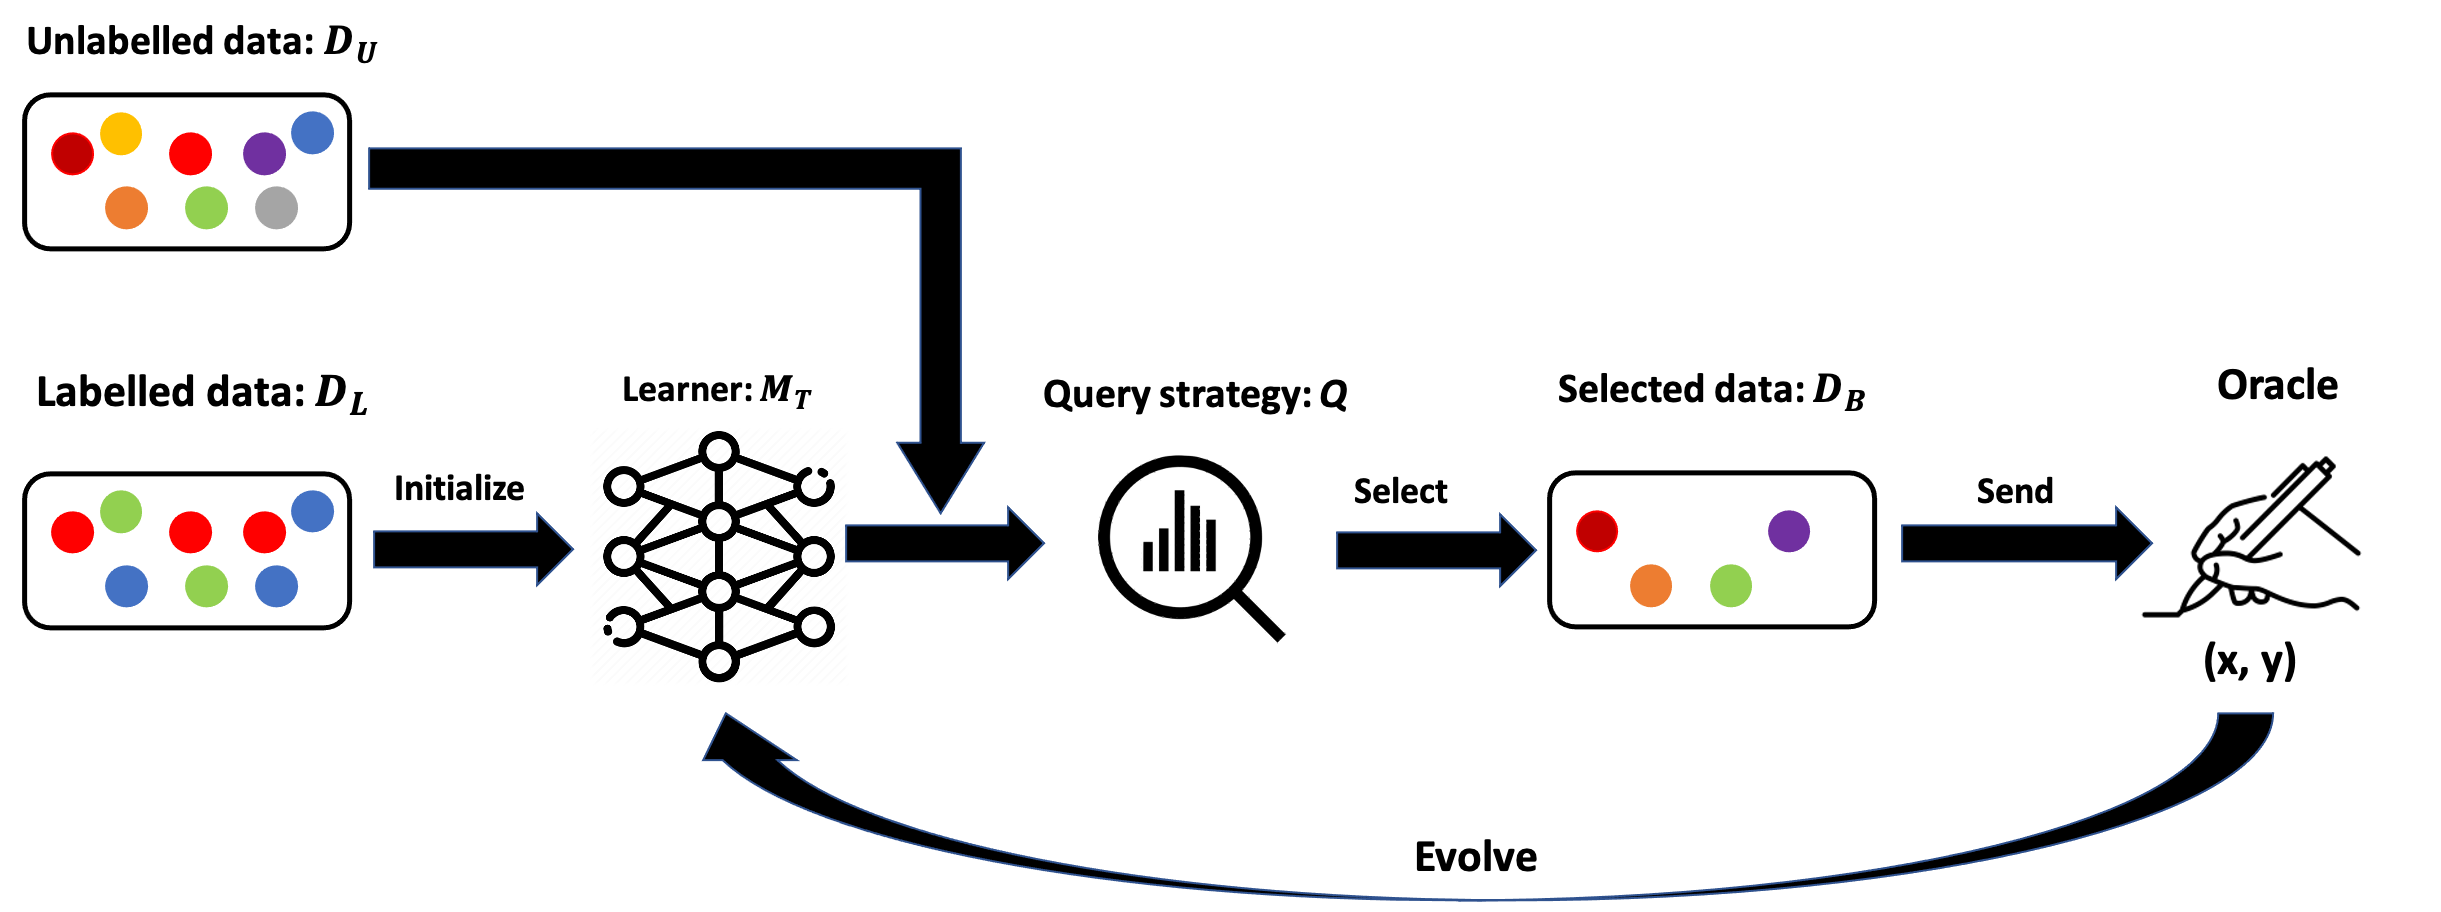
\includegraphics[width=\textwidth]{images/al_framework.png}
    \caption{AL framework}
    \label{fig:framework}
\end{figure}



{\noindent \em Remainder omitted in this sample. See http://www.jmlr.org/papers/ for full paper.}

% Acknowledgements should go at the end, before appendices and references

\acks{We would like to acknowledge support for this project
from the National Science Foundation (NSF grant IIS-9988642)
and the Multidisciplinary Research Program of the Department
of Defense (MURI N00014-00-1-0637). }



\newpage

\appendix
\section*{Appendix A.}
\label{app:theorem}

% Note: in this sample, the section number is hard-coded in. Following
% proper LaTeX conventions, it should properly be coded as a reference:

%In this appendix we prove the following theorem from
%Section~\ref{sec:textree-generalization}:

In this appendix we prove the following theorem from
Section~6.2:

\noindent
{\bf Theorem} {\it Let $u,v,w$ be discrete variables such that $v, w$ do
not co-occur with $u$ (i.e., $u\neq0\;\Rightarrow \;v=w=0$ in a given
dataset $\dataset$). Let $N_{v0},N_{w0}$ be the number of data points for
which $v=0, w=0$ respectively, and let $I_{uv},I_{uw}$ be the
respective empirical mutual information values based on the sample
$\dataset$. Then
\[
	N_{v0} \;>\; N_{w0}\;\;\Rightarrow\;\;I_{uv} \;\leq\;I_{uw}
\]
with equality only if $u$ is identically 0.} \hfill\BlackBox

\noindent
{\bf Proof}. We use the notation:
\[
P_v(i) \;=\;\frac{N_v^i}{N},\;\;\;i \neq 0;\;\;\;
P_{v0}\;\equiv\;P_v(0)\; = \;1 - \sum_{i\neq 0}P_v(i).
\]
These values represent the (empirical) probabilities of $v$
taking value $i\neq 0$ and 0 respectively.  Entropies will be denoted
by $H$. We aim to show that $\fracpartial{I_{uv}}{P_{v0}} < 0$....\\

{\noindent \em Remainder omitted in this sample. See http://www.jmlr.org/papers/ for full paper.}


\vskip 0.2in
\bibliography{ref}

\end{document}
